\documentclass[11pt]{article}
\usepackage[utf8]{inputenc}

%%% PAGE DIMENSIONS
\usepackage{geometry}
\geometry{a4paper}

\usepackage{graphicx}

%%% PACKAGES
\usepackage{booktabs}
\usepackage{paralist}
\usepackage{verbatim}
\usepackage{subfig}
\usepackage{chngcntr}
\usepackage{tikz}
\usepackage[colorlinks = true,
            linkcolor = black,
            urlcolor  = blue,
            citecolor = blue,
            anchorcolor = blue]{hyperref}
\usepackage[spanish]{cleveref}
\usepackage{placeins}
\usepackage{float}
\usepackage{listings}

%%% HEADERS & FOOTERS
\usepackage{fancyhdr}
\pagestyle{fancy}
\renewcommand{\headrulewidth}{0pt}
\lhead{}\chead{}\rhead{}
\lfoot{}\cfoot{\thepage}\rfoot{}

%%% SECTION TITLE APPEARANCE
\usepackage{sectsty}
\allsectionsfont{\sffamily\mdseries\upshape}

%%% ToC (table of contents) APPEARANCE
\usepackage[nottoc,notlof,notlot]{tocbibind} % Put the bibliography in the ToC
\usepackage[titles,subfigure]{tocloft} % Alter the style of the Table of Contents
\renewcommand{\cftsecfont}{\rmfamily\mdseries\upshape}
\renewcommand{\cftsecpagefont}{\rmfamily\mdseries\upshape} % No bold!


\graphicspath{ {images/} }

\counterwithin*{figure}{section}
\counterwithin*{figure}{subsection}
\counterwithin*{figure}{subsubsection}

\counterwithin*{table}{section}
\counterwithin*{table}{subsection}
\counterwithin*{table}{subsubsection}

\addtolength{\cftfignumwidth}{2em}

\renewcommand{\thefigure}{
  \ifnum\value{subsection}=0
    \thesection.\arabic{figure}
  \else
    \ifnum\value{subsubsection}=0
      \thesubsection.\arabic{figure}
    \else
      \thesubsubsection.\arabic{figure}
    \fi
  \fi
}

\renewcommand{\thetable}{
  \ifnum\value{subsection}=0
    \thesection.\arabic{table}
  \else
    \ifnum\value{subsubsection}=0
      \thesubsection.\arabic{table}
    \else
      \thesubsubsection.\arabic{table}
    \fi
  \fi
}

%%% END Article customizations

%%% The "real" document content comes below...

\title{\Large Seguridad en Redes\\Practica 3.5}
\author{David Antuña Rodríguez\\Javier Carrión García}
\date{}

\begin{document}
  \raggedright

  \maketitle
  \newpage

  \section{Conexión IPsec de sitio a sitio con clave secreta}
    \par
    Registros del fichero \textit{/var/log/daemon.log}
    \lstset{basicstyle=\ttfamily\tiny}
\begin{lstlisting}
xcbc hmac ctr ccm gcm attr kernel-netlink resolve socket-raw farp stroke updown eap-identity eap-aka eap-md5 eap-gtc
    eap-mschapv2 eap-radius eap-tls eap-ttls eap-tnc dhcp led addrblock
Apr 14 13:39:10 debian charon: 00[JOB] spawning 16 worker threads
Apr 14 13:42:16 debian charon: 00[DMN] signal of type SIGINT received. Shutting down
Apr 14 13:42:19 debian charon: 00[DMN] Starting IKEv2 charon daemon (strongSwan 4.5.2)
Apr 14 13:42:19 debian charon: 00[KNL] listening on interfaces:
Apr 14 13:42:19 debian charon: 00[KNL]   eth0
Apr 14 13:42:19 debian charon: 00[KNL]     10.0.2.15
Apr 14 13:42:19 debian charon: 00[KNL]     fe80::a00:27ff:febe:6b91
Apr 14 13:42:19 debian charon: 00[KNL]   eth1
Apr 14 13:42:19 debian charon: 00[KNL]     192.168.1.1
Apr 14 13:42:19 debian charon: 00[KNL]     fe80::a00:27ff:fe66:bfba
Apr 14 13:42:19 debian charon: 00[KNL]   eth2
Apr 14 13:42:19 debian charon: 00[KNL]     192.168.3.1
Apr 14 13:42:19 debian charon: 00[KNL]     fe80::a00:27ff:fe99:5f2b
Apr 14 13:42:19 debian charon: 00[CFG] loading ca certificates from '/etc/ipsec.d/cacerts'
Apr 14 13:42:19 debian charon: 00[CFG] loading aa certificates from '/etc/ipsec.d/aacerts'
Apr 14 13:42:19 debian charon: 00[CFG] loading ocsp signer certificates from '/etc/ipsec.d/ocspcerts'
Apr 14 13:42:19 debian charon: 00[CFG] loading attribute certificates from '/etc/ipsec.d/acerts'
Apr 14 13:42:19 debian charon: 00[CFG] loading crls from '/etc/ipsec.d/crls'
Apr 14 13:42:19 debian charon: 00[CFG] loading secrets from '/etc/ipsec.secrets'
Apr 14 13:42:19 debian charon: 00[CFG] expanding file expression '/var/lib/strongswan/ipsec.secrets.inc' failed
Apr 14 13:42:19 debian charon: 00[CFG]   loaded IKE secret for %any
Apr 14 13:42:19 debian charon: 00[CFG] sql plugin: database URI not set
Apr 14 13:42:19 debian charon: 00[LIB] plugin 'sql': failed to load - sql_plugin_create returned NULL
Apr 14 13:42:19 debian charon: 00[CFG] loaded 0 RADIUS server configurations
Apr 14 13:42:19 debian charon: 00[LIB] plugin 'medsrv' failed to load: /usr/lib/ipsec/plugins/libstrongswan-medsrv.so:
    cannot open shared object file: No such file or directory
Apr 14 13:42:19 debian charon: 00[CFG] mediation client database URI not defined, skipped
Apr 14 13:42:19 debian charon: 00[LIB] plugin 'medcli': failed to load - medcli_plugin_create returned NULL
Apr 14 13:42:19 debian charon: 00[LIB] plugin 'nm' failed to load: /usr/lib/ipsec/plugins/libstrongswan-nm.so: cannot
    open shared object file: No such file or directory
Apr 14 13:42:19 debian charon: 00[CFG] HA config misses local/remote address
Apr 14 13:42:19 debian charon: 00[LIB] plugin 'ha': failed to load - ha_plugin_create returned NULL
Apr 14 13:42:19 debian charon: 00[DMN] loaded plugins: test-vectors curl ldap aes des sha1 sha2 md5 random x509
    revocation constraints pubkey pkcs1 pgp pem openssl fips-prf gmp agent pkcs11 xcbc hmac ctr ccm gcm attr
    kernel-netlink resolve socket-raw farp stroke updown eap-identity eap-aka eap-md5 eap-gtc eap-mschapv2 eap-radius
    eap-tls eap-ttls eap-tnc dhcp led addrblock
Apr 14 13:42:19 debian charon: 00[JOB] spawning 16 worker threads
Apr 14 13:42:19 debian charon: 11[CFG] received stroke: add connection 'secret'
Apr 14 13:42:19 debian charon: 11[CFG] added configuration 'secret'
Apr 14 13:43:54 debian charon: 11[CFG] received stroke: initiate 'secret'
Apr 14 13:43:54 debian charon: 04[IKE] initiating IKE_SA secret[1] to 192.168.3.2
Apr 14 13:43:54 debian charon: 04[ENC] generating IKE_SA_INIT request 0 [ SA KE No N(NATD_S_IP) N(NATD_D_IP) ]
Apr 14 13:43:54 debian charon: 04[NET] sending packet: from 192.168.3.1[500] to 192.168.3.2[500]
Apr 14 13:43:54 debian charon: 03[NET] received packet: from 192.168.3.2[500] to 192.168.3.1[500]
Apr 14 13:43:54 debian charon: 03[ENC] parsed IKE_SA_INIT response 0 [ SA KE No N(NATD_S_IP) N(NATD_D_IP) N(MULT_AUTH) ]
Apr 14 13:43:54 debian charon: 03[IKE] authentication of '192.168.3.1' (myself) with pre-shared key
Apr 14 13:43:54 debian charon: 03[IKE] establishing CHILD_SA secret
Apr 14 13:43:54 debian charon: 03[ENC] generating IKE_AUTH request 1 [ IDi N(INIT_CONTACT) IDr AUTH SA TSi TSr N(MOBIKE_SUP)
    N(ADD_4_ADDR) N(ADD_4_ADDR) N(MULT_AUTH) N(EAP_ONLY) ]
Apr 14 13:43:54 debian charon: 03[NET] sending packet: from 192.168.3.1[4500] to 192.168.3.2[4500]
Apr 14 13:43:54 debian charon: 02[NET] received packet: from 192.168.3.2[4500] to 192.168.3.1[4500]
Apr 14 13:43:54 debian charon: 02[ENC] parsed IKE_AUTH response 1 [ IDr AUTH SA TSi TSr N(AUTH_LFT) N(MOBIKE_SUP)
    N(ADD_4_ADDR) N(ADD_4_ADDR) ]
Apr 14 13:43:54 debian charon: 02[IKE] authentication of '192.168.3.2' with pre-shared key successful
Apr 14 13:43:54 debian charon: 02[IKE] IKE_SA secret[1] established between 192.168.3.1[192.168.3.1]...192.168.3.2[192.168.3.2]
Apr 14 13:43:54 debian charon: 02[IKE] scheduling reauthentication in 9764s
Apr 14 13:43:54 debian charon: 02[IKE] maximum IKE_SA lifetime 10304s
Apr 14 13:43:54 debian charon: 02[IKE] CHILD_SA secret{1} established with SPIs c52f9e44_i c1e4762b_o and TS 192.168.1.0/24 ===
    192.168.2.0/24
Apr 14 13:43:54 debian charon: 02[IKE] received AUTH_LIFETIME of 9883s, scheduling reauthentication in 9343s
Apr 14 13:43:54 debian charon: 02[IKE] peer supports MOBIKE
\end{lstlisting}

    \begin{figure}[H]
      \centering
      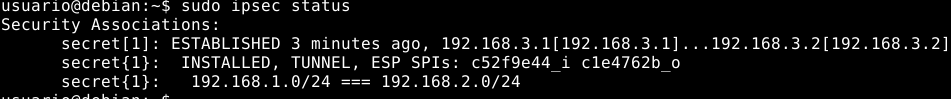
\includegraphics[width = \textwidth]{IPSstatus}
      \caption{Detalles de la conexión.}
    \end{figure}

    \par
    Como se puede ver en la figura \ref{fig:secasoc}hay dos asociaciones de
    seguridad, una por cada sentido de la conexión. Almacena la firma y la clave
    de encriptación.
    \begin{figure}[H]
      \centering
      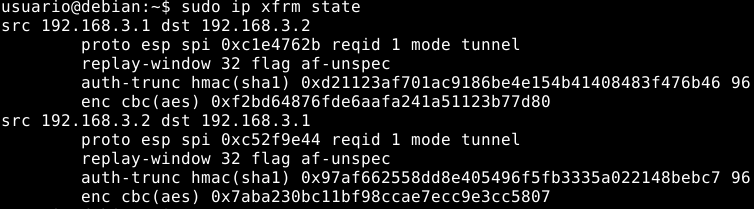
\includegraphics[width = \textwidth]{asocSec}
      \caption{Asociaciones de seguridad.}
      \label{fig:secasoc}
    \end{figure}

    \par
    Hay tres politicas según el paquete.
    \begin{itemize}
      \item Si se retransmite (fwd).
      \item Si va dirigido a la maquina (in)
      \item Si lo emite la maquina (out)
    \end{itemize}

    \par
    Todo el tráfico aplicará la acción PROTECT.

    \begin{figure}[H]
      \centering
      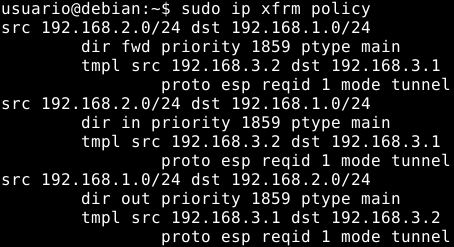
\includegraphics[width = .8\textwidth]{policy}
      \caption{Políticas de seguridad.}
    \end{figure}

    \par
    Se han intercambiado 4 paquetes ISAKMP como se puede ver en la figura
    \ref{fig:packisak}. Esta usando la version 2.0, se puede ver al inspeccionar
    el paquete (figura \ref{fig:visak}).

    \begin{figure}[H]
      \centering
      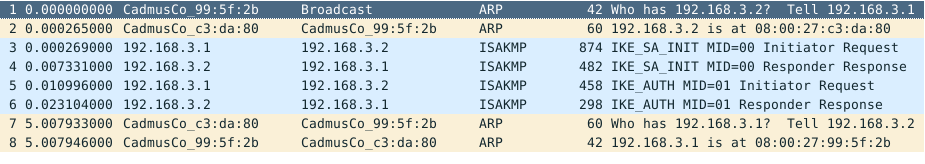
\includegraphics[width = \textwidth]{packisak}
      \caption{Paquetes ISAKMP capturados.}
      \label{fig:packisak}
    \end{figure}

    \begin{figure}[H]
      \centering
      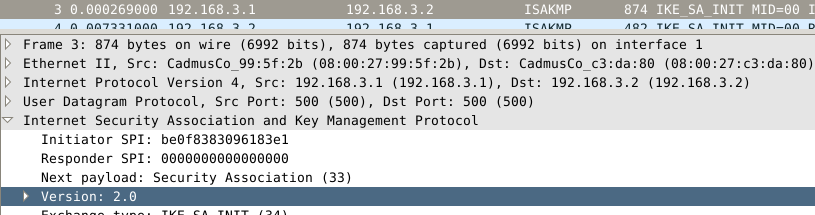
\includegraphics[width = \textwidth]{visak}
      \caption{Version ISAKMP.}
      \label{fig:visak}
    \end{figure}

    \par
    Si miramos de nuevo la figura \ref{fig:visak} podemos ver que utiliza User
    Datagram Protocol (UDP) y el puerto asociado es el 500.

    \bigskip
    \par
    Si inspeccionamos el paquete podemos ver que han acordado usar cbc con aes
    y que el tamaño de la clave es 128, figura \ref{fig:alg}.

    \begin{figure}[H]
      \centering
      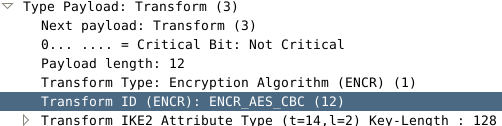
\includegraphics[width = \textwidth]{alg}
      \caption{Acuerdo.}
      \label{fig:alg}
    \end{figure}

    \par
    Va a usar SHA1, figura \ref{fig:prf}, con el grupo DH 14(2048 bit modulus),
    figura \ref{fig:dh}.

    \begin{figure}[H]
      \centering
      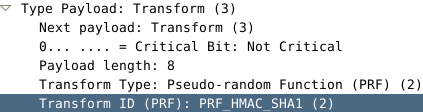
\includegraphics[width = \textwidth]{prf}
      \caption{Pseudo Random Function (PRF).}
      \label{fig:prf}
    \end{figure}

    \begin{figure}[H]
      \centering
      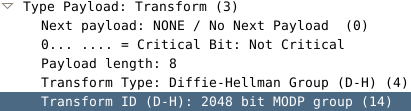
\includegraphics[width = \textwidth]{dh}
      \caption{Grupo DH.}
      \label{fig:dh}
    \end{figure}

    \par
    El segundo par de mensajes se usan para autenticar ambos extremos, un
    atacante no puede ver los datos intercambiados porque van cifrados con lo
    que se ha acordado por ambos extremos en los dos mensajes previos.

    \begin{figure}[H]
      \centering
      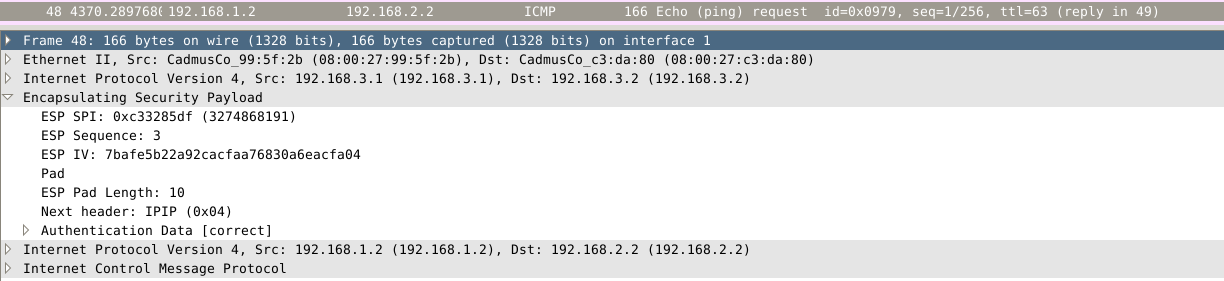
\includegraphics[width = \textwidth]{espdcipher}
      \caption{Paquete ESP descifrado.}
    \end{figure}

    \par
    Como se puede ver en la figura \ref{fig:espcfg} no se comparte ni el SPI ni
    las claves.

    \begin{figure}[H]
      \centering
      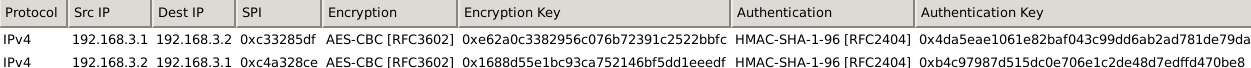
\includegraphics[width = \textwidth]{espcfg}
      \caption{Parámetros SAs.}
      \label{fig:espcfg}
    \end{figure}

    \par
    El encapsulado ESP en modo tunel añade una cabecera IP nueva de modo que
    todo lo que la siga va firmado, además lo que sigue a la cabecera ESP
    va también encriptado.

  \section{Conexión IPsec de sitio a sitio con certificado autofirmado}
    \begin{figure}[H]
      \centering
      \hspace*{-.5in}
      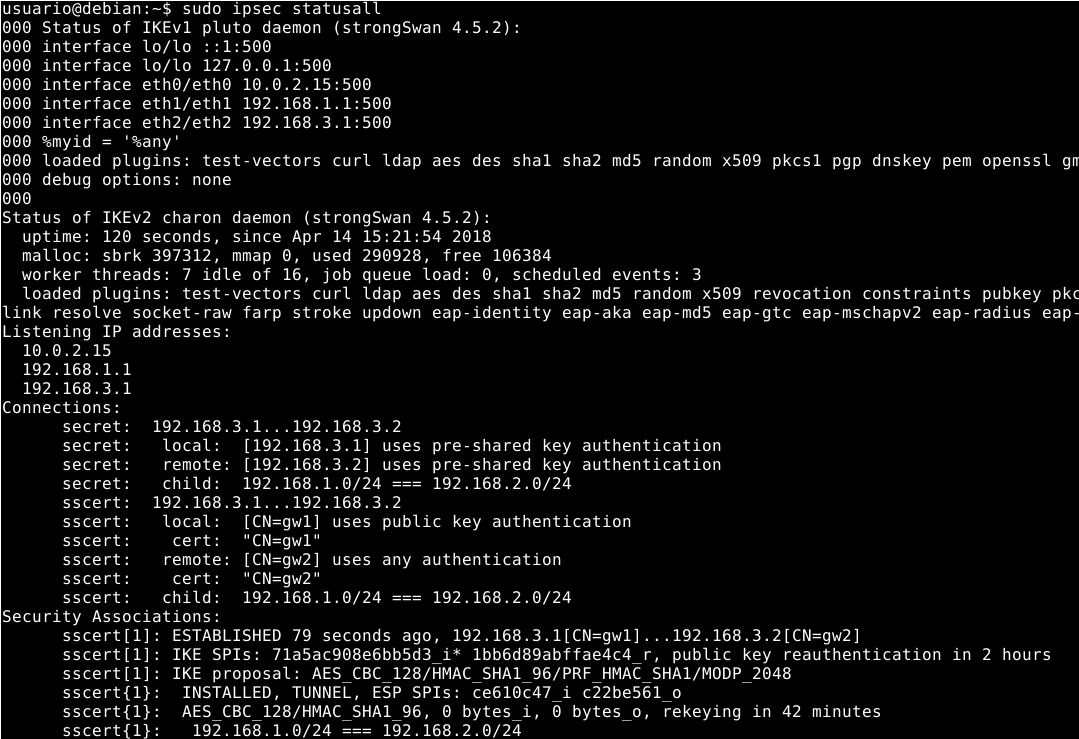
\includegraphics[width = 1.2\textwidth]{statusall}
      \caption{sudo ipsec statusall}
    \end{figure}

    \par
    El establecimiento es igual, solo cambia el método de autenticación.
\end{document}
